\chapter{Conclusão}\label{chp:conclusao}

\section{Introdução}\label{sec:conclusao-introducao}
Neste capítulo apresentamos algumas considerações finais a respeito deste projeto, tais como reflexões sobre a motivação, busca da solução e conclusão sobre o seu desenvolvimento. Além disso, sugerimos algumas novas funcionalidades e melhorias como trabalhos futuros, para que este projeto continue sendo desenvolvido e cada vez mais se torne uma alternativa viável na automatização e gestão de processos de negócio.

\section{Considerações}\label{sec:conclusao-introducao}

O combustível principal deste trabalho, fortemente compartilhado por todos os seus integrantes, foi a possibilidade de unir o interesse acadêmico e a incrível experiência vivenciada durante todos os anos de estudos na UFRJ com o objetivo de gerar valor para o mercado corporativo através da Visagio\cite{visagio}, empresa na qual trabalhamos há mais de três anos e formada por ex-alunos desta instituição.

Tendo iniciado com a necessidade de automatizar e padronizar processos simples e com bastante interação humana, encontramos no Redmine uma ótima solução. Descobrimos que o Gerenciador de Projetos podia também ser utilizado como Gerenciador de Processos. Utilizar este sistema faz sentido pela excelente estrutura de gerenciamento de tarefas, acompanhamento do histórico, facilidade para criação de fluxos de trabalho, campos personalizados, e ótimo controle de permissões.

Contudo, se quisermos guiar processos mais complexos, com fluxos paralelos, atribuições, ou decisões de caminhos automáticas, o Redmine por si só não nos atenderia. Ele não foi desenvolvido originalmente com este objetivo, e não valeria a pena tentar desenvolver plugins para possibilitar a condução de processos complexos no Redmine, pois as funcionalidades que são necessárias para isto, já foram todas implementadas em sistemas chamados BPMS.

Os BPMS foram desenvolvidos exatamente com o objetivo de modelar fluxos complexos, e nos atenderiam muito bem em termos de execução do processo. No entanto, como uma das características dos processos que queremos poder automatizar é a necessidade de bastante interação humana, todas as funcionalidades que facilitam esta interação do Redmine citadas acima, nos fariam falta, pois este não é o foco dos BPMS.

A proposta final deste trabalho portanto foi o desenvolvimento de um plugin para o Redmine, que chamamos de \textit{BPM Integration}, para integrá-lo com um BPMS. Como descrevemos no Capítulo \ref{chp:integracao_redmine_activiti}, a abordagem inicial foi utilizar um ESB\cite{esb} como uma camada de comunicação entre o Redmine e os BPMS, e desenvolver uma plataforma genérica à qual pudesse ser plugado qualquer BPMS. Devido a algumas dificuldades nesta estratégica, decidimos estabelecer a comunicação com apenas um BPMS e após avaliarmos as possibilidades disponíveis, escolhemos o Activiti BPM\cite{bpm_activiti}.

O plugin \textit{BPM Integration} foi desenvolvido em Ruby on Rails, a linguagem na qual o Redmine foi feito. Ademais, a comunicação entre o Redmine e o Activiti BPM foi feita através do consumo da API REST disponibilizada pelo último.


\section{Melhorias Propostas}\label{sec:conclusao-melhorias}

Em alinhamento com a utilização de soluções de código-fonte aberto que compõem este trabalho, todo o código-fonte da integração desenvolvida está disponibilizado no GitHub da Visagio\cite{github_visagio}. O \textit{Redmine BPM Integration Plugin} segue em constante evolução através da implementação desta solução em clientes relevantes no Brasil, o que exige constantes melhorias e avanços no projeto inicial apresentado neste trabalho.

A seguir são apresentadas algumas propostas de melhorias para o seguimento deste trabalho:

\subsection{Tarefas Contínuas}

Durante a implantação, um \textit{feedback} foi recebido pelos usuários do sistema. O plugin introduziu um comportamento um pouco diferente na continuidade do processo do que era de costume no Redmine. Como explicado na Seção \ref{sec:integracao_redmine_activiti_sincronizacao-criacao_human_task}, a representação de uma tarefa humana do Activiti no Redmine é uma sub-tarefa do chamado original que representa o processo. Uma das principais razões desta abordagem foi a necessidade de contemplar processos que existem tarefas humanas que devem ser realizadas em paralelo, de modo que cada ator pudesse executar sua tarefa isoladamente numa sub-tarefa. 

Esta modificação, no entanto, tirou um pouco a continuidade de um processo em que várias etapas são executadas sequencialmente por um mesmo ator. Na condução de um processo no Redmine sem o plugin \textit{BPM Integration} os atores sempre interagem com o processo através da tarefa que representa o mesmo no Redmine. 

Já na modelagem proposta com o plugin \textit{BPM Integration} o usuário interage com o processo através da sub-tarefa atribuída para ele e altera a situação desta, representando a conclusão daquela etapa. Ao fazer isto o processo segue para a próxima etapa no Activiti BPM e cria a próxima atividade (\ref{sec:bpm-bpmn_objetos_fluxo}) e o plugin \textit{BPM Integration} em seguida cria uma nova sub-tarefa, para permitir a interação do ator com o processo, através do Redmine. 

Quando o usuário conclui uma sub-tarefa, e ele é o responsável pela próxima etapa, ele não visualiza imediatamente na tela a próxima sub-tarefa criada, permitindo que avance as etapas numa mesma tela. Nestes casos é necessário acessar a tarefa pai da sub-tarefa que acabou de ser concluída (a que representa o processo), e à partir daí, acessar a próxima sub-tarefa. Neste cenário, existe possibilidade de melhorias para facilitar a execução das tarefas para o usuário, permitindo que o processo flua melhor quando as tarefas sequenciais são executadas por um mesmo ator.

As Figuras \ref{fig:acessar_subtarefa} e \ref{fig:acessar_tarefa_pai} mostram como é o acesso às tarefas mencionado acima, exemplificado com o processo de criação de cartões corporativos ilustrado na Figura \ref{fig:process_cartao_compras}. Após concluir a tarefa, o usuário deve clicar no link em amarelo na parte superior da tela exibida na Figura \ref{fig:acessar_tarefa_pai}. Ao fazer isto é redirecionado para a tela da tarefa que representa o processo, exibida na Figura \ref{fig:acessar_subtarefa}. Abaixo do título \textit{Sub-chamados} estão as sub-tarefas. Como é possível observar, a primeira sub-tarefa é a que acabou de ser concluída, com a situação \textit{Aprovado}, e a segunda é a próxima etapa a ser realizada, em cujo link o ator deve clicar para acessá-la.

\begin{figure}[H]
\centering
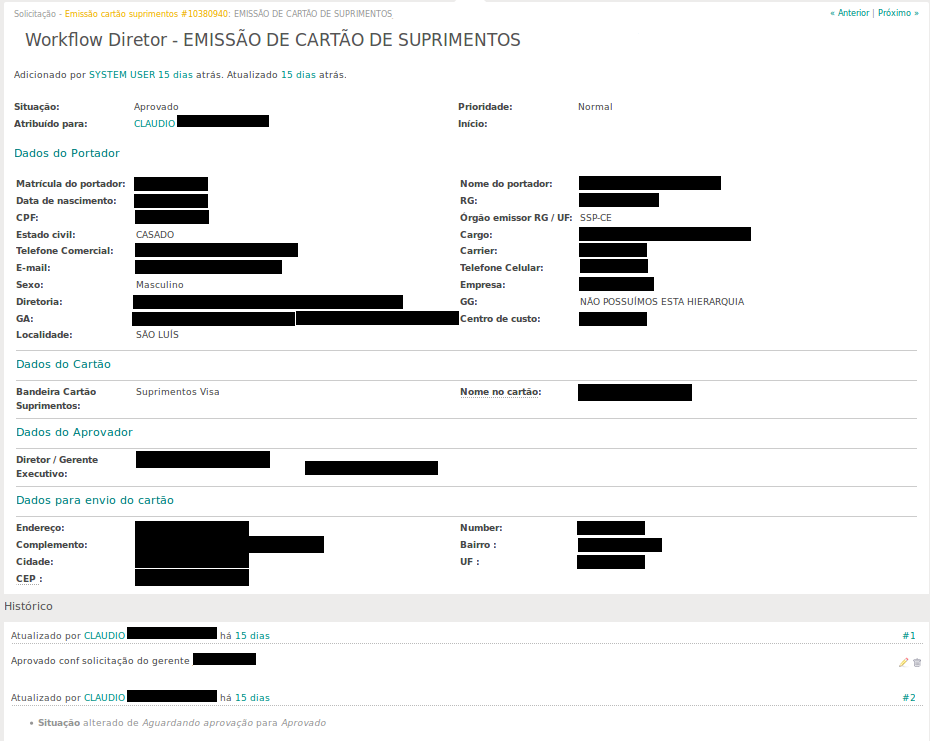
\includegraphics[width=1\textwidth]{imagens/acessar_tarefa_pai.png}
\caption{Sub-tarefa, representando uma das etapas do processo de criação de cartões corporativos}
\label{fig:acessar_tarefa_pai}
\end{figure}

\begin{figure}[H]
\centering
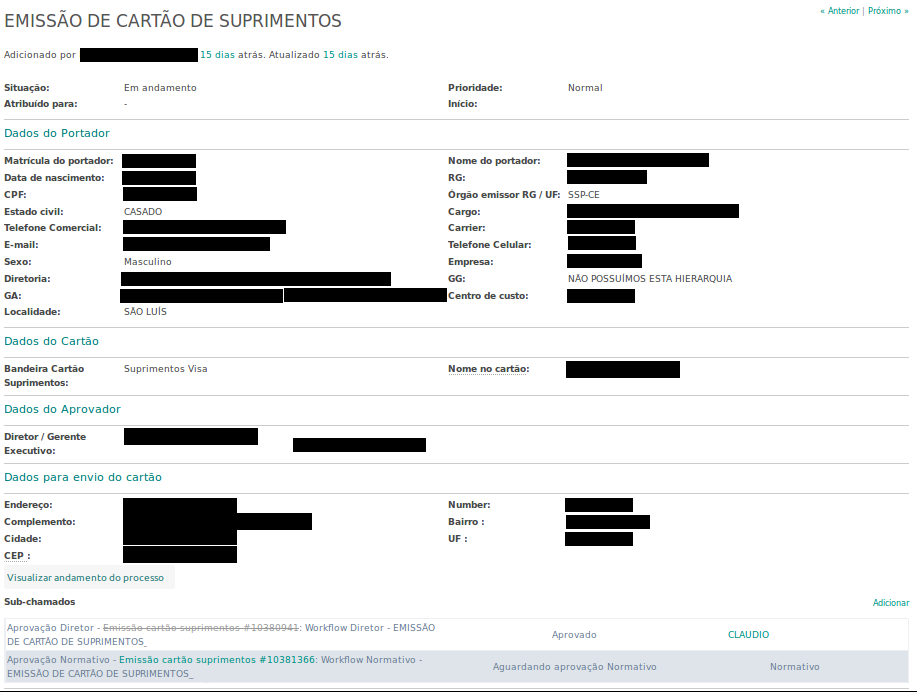
\includegraphics[width=1\textwidth]{imagens/acessar_subtarefa.png}
\caption{Tarefa representando o processo de criação de cartões corporativos}
\label{fig:acessar_subtarefa}
\end{figure}

\subsection{BPMN Integrado}

Neste trabalho utilizamos o Activiti Designer para a modelagem dos processos que é constituído basicamente do Eclipse com um plugin BPMN. Este cenário apresenta-se pouco prático para usuários sem conhecimento de TI. Nesse sentido, observamos a oportunidade de prover uma modelagem de processos fácil e integrada ao Redmine. Assim, o usuário poderia criar seu processo diretamente na ferramenta, com uma interface simples e online, sem a necessidade de contato com aplicações específicas de desenvolvimento.

Já existem iniciativas similares neste sentido, como o Activiti Modeler\cite{activiti_modeler}, exibido na Figura \ref{fig:activiti_modeler}. Portanto, uma melhoria interessante seria acoplar esta ferramenta ao Redmine e avaliar as melhorias necessárias para deixar sua utilização agradável e simples numa única ferramenta.

\begin{figure}[H]
\centering
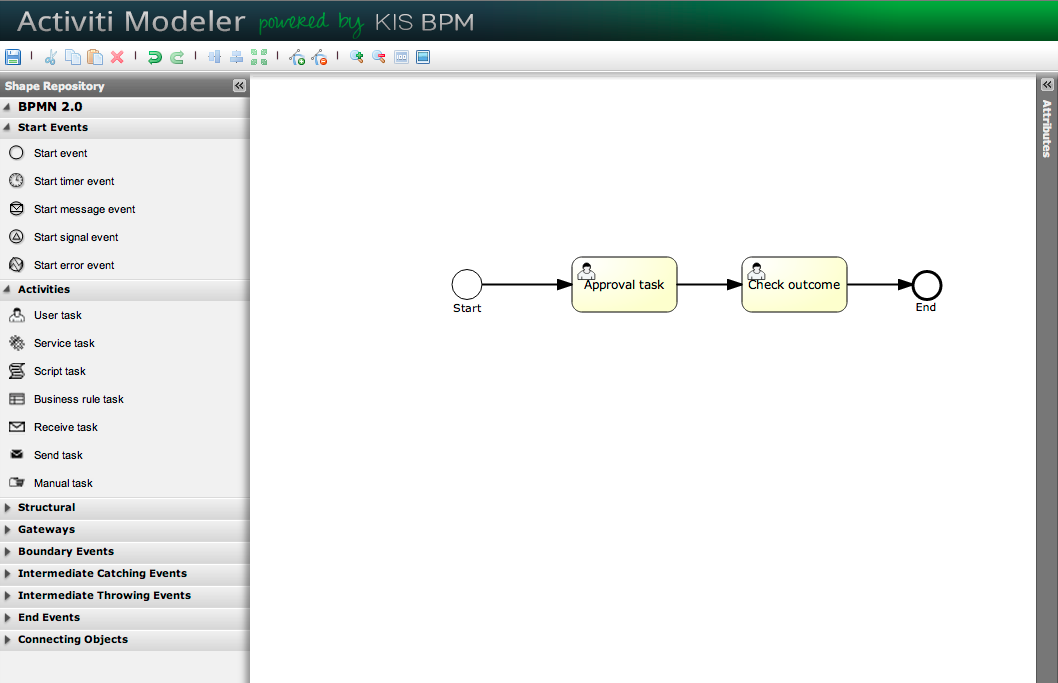
\includegraphics[width=1\textwidth]{imagens/activiti_modeler.png}
\caption{Activiti Modeler}
\label{fig:activiti_modeler}
\end{figure}

\subsection{BRM Integrado}

Uma característica bastante comum em sistemas BPMS é a presença de um BRM (\textit{Business Rules Management}) para gestão de regras de negócio nos processos. O Activiti BPM suporta a integração com o Drools, uma aplicação \textit{web} desenvolvida em Java especialista em BRM. O Drools permite a criação de uma tabela de decisão que pode ser configurada pelo usuário para definir uma regra de negócio baseada em intervalo de valores estabelecendo, por exemplo, as alçadas de aprovação em um processo de pagamento.

Uma proposta de evolução no contexto da integração do BPMS com o Redmine seria o desenvolvimento de um plugin BRM que permita a gestão de regras de negócio para processos BPM diretamente no Redmine.

\subsection{BPMS Genérico}

Conforme discutido na Seção \ref{sec:cenario-integracao-genérica}, esta melhoria proporcionaria uma camada genérica de integração de qualquer BPMS ao Redmine, flexibilizando assim a escolha do BPMS ou até mesmo a integração com um BPMS que já esteja em uso pela empresa. 